\documentclass[tikz,border=3pt]{standalone}
\usetikzlibrary{arrows.meta,positioning}
\begin{document}
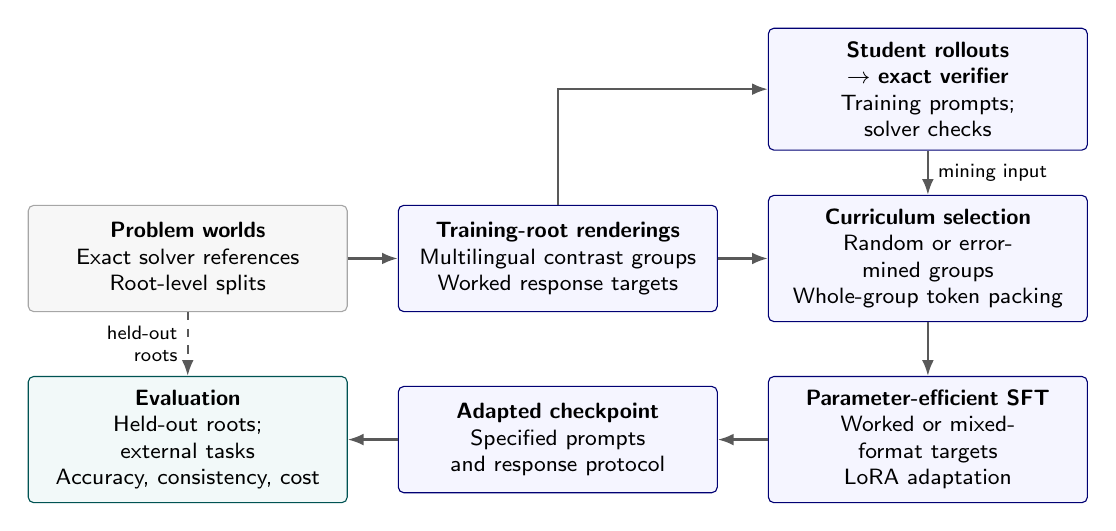
\begin{tikzpicture}[
  font={\sffamily\footnotesize},
  box/.style={draw=black!35,rounded corners=2pt,fill=black!3,align=center,text width=3.7cm,minimum height=1.35cm,inner sep=5pt},
  train/.style={box,draw=blue!45!black,fill=blue!4},
  test/.style={box,draw=teal!65!black,fill=teal!5},
  arrow/.style={-{Latex[length=2mm]},thick,draw=black!65}]
\node[box] (world) at (0,0) {\textbf{Problem worlds}\\Exact solver references\\Root-level splits};
\node[train] (render) at (4.7,0) {\textbf{Training-root renderings}\\Multilingual contrast groups\\Worked response targets};
\node[train] (select) at (9.4,0) {\textbf{Curriculum selection}\\Random or error-mined groups\\Whole-group token packing};
\node[test] (eval) at (0,-2.3) {\textbf{Evaluation}\\Held-out roots; external tasks\\Accuracy, consistency, cost};
\node[train] (model) at (4.7,-2.3) {\textbf{Adapted checkpoint}\\Specified prompts\\and response protocol};
\node[train] (fit) at (9.4,-2.3) {\textbf{Parameter-efficient SFT}\\Worked or mixed-format targets\\LoRA adaptation};
\node[train,minimum height=1.05cm] (verify) at (9.4,2.15) {\textbf{Student rollouts $\rightarrow$ exact verifier}\\Training prompts; solver checks};
\draw[arrow] (render.north) |- (verify.west);
\draw[arrow] (verify.south) -- node[right,font=\sffamily\scriptsize] {mining input} (select.north);
\draw[arrow] (world) -- (render);
\draw[arrow] (render) -- (select);
\draw[arrow] (select) -- (fit);
\draw[arrow] (fit) -- (model);
\draw[arrow] (model) -- (eval);
\draw[arrow,dashed] (world) -- node[left,align=right,font=\sffamily\scriptsize] {held-out\\roots} (eval);
\end{tikzpicture}
\end{document}
